% =============================================================================
%  LOWER VOLUME: Articles 43--85 and Historical Price Records
%  Source: translation/pages_79-82.md, pages_83-86.md,
%          pages_87-90.md, pages_91-94.md
% =============================================================================

% --- Article 43 ---
\article{43}{Five Articles on the Osaka Market}

\begin{sokyubox}
{\small\itshape\color{sokyubar} \jp{第四十三章\quad 大阪相塲五ケ條の事}}

\medskip
The Osaka market price around the twenty-seventh or twenty-eighth of the
ninth month reflects the crop conditions of the eastern provinces, which
by then are broadly known.

The Osaka market's contract changeover (\jt{立代り}{tachikawari}) falls
on the seventeenth of the tenth month. Prices through around the twentieth
are dispatched, arriving here around the sixth of the eleventh month.

The Osaka grand settlement price (\jt{大調べ}{\=oshirabe}) on the
eleventh of the twelfth month arrives around the twenty-seventh or
twenty-eighth of that month.

The Osaka year-end rice price and the fourth-day opening market price
arrive around the twenty-fourth or twenty-fifth of the first month.

The Osaka market's contract changeover on the seventh of the fifth
month: prices through about the tenth are dispatched, arriving around the
twenty-third or twenty-fourth of the fifth month.
\end{sokyubox}

\commentary
The articles above record the number of days required for Osaka market
prices to reach Sakata. In the master's time, transportation was not yet
as developed as it is today, and all market intelligence was communicated
by entrusting written dispatches to express couriers (\jt{飛脚}{hikyaku}).
As the text shows, Osaka prices required between sixteen and roughly
twenty days to become known in Sakata.

% --- Article 44 ---
\article{44}{On Higo Rice as a Leading Commodity}

\begin{sokyubox}
{\small\itshape\color{sokyubar} \jp{第四十四章\quad 肥後米立物の事}}

\medskip
In a year when Higo rice (\jt{肥後米}{Higo-mai}) becomes the leading
commodity (\jt{立物}{tatemono}), price swings are violent and the market
is generally biased upward. When prices climb to their limit, the reversal
is extremely swift. It is a rice that permits no complacency.
\end{sokyubox}

% --- Article 45 ---
\article{45}{On Those Who Move Funds Easily and Those Who Are Constrained}

\begin{sokyubox}
{\small\itshape\color{sokyubar} \jp{第四十五章\quad 米金差繰易き人並に不自由なる人の事}}

\medskip
Those who can readily shift between rice and money (\jt{米金差繰}{bekin-sakuri})
are inclined toward the buy side. Those whose rice-and-money position is
constrained invariably lean toward the sell side. For this reason, even a
small rise sends them scrambling to buy back their positions.
\end{sokyubox}

\commentary
``Rice-money freedom'' (\jt{米金自由}{bekin jiy\=u}) refers to a commercial
custom of the Sh\=onai region: a fixed term is agreed upon, during which
one party has free use of rice and the other has free use of money; when
the term expires, each returns what was borrowed in its original form.

The meaning of this chapter is as follows: those who can easily manage the
shifting between rice and money---that is, those with ready access to
funds---tend naturally toward the buy side. Those whose rice-and-money
position is constrained tend to side with the sellers. For this reason,
even a small rise throws them into panic, and they scramble to buy back
their short positions.

% --- Article 46 ---
\article{46}{On Times When Gold Piles High}

\begin{sokyubox}
{\small\itshape\color{sokyubar} \jp{第四十六章\quad 金澤山成時の事}}

\medskip
When gold is plentiful (\jt{金澤山}{kane takusan}), rice tends to be
cheap. This is because there is little speculative interest in rice, and
funds flow into interest-bearing deposits (\jt{歩金}{bukin}). When gold
is scarce, rice is dear. This is because speculative interest in rice is
strong.
\end{sokyubox}

\commentary
In today's world, with its developed financial institutions, it is obvious
that when currency is abundant, commodity prices rise. But this chapter
observes from within the feudal era, and specifically from the extremely
narrow vantage of the Sh\=onai region.

The meaning is this: when gold appears plentiful in the local market, it is
because speculative interest (\jt{思入}{omoiire}) in rice is low and funds
have flowed out as interest deposits. Consequently, the market is cheap.
Conversely, when one looks into why circulating money is scarce in the
market, it is because speculative interest in rice is strong and funds have
been committed to rice positions. Consequently, the market is dear.

% --- Article 47 ---
\article{47}{On Years When Winter Purchases Do or Do Not Reach the Shippers}

\begin{sokyubox}
{\small\itshape\color{sokyubar} \jp{第四十七章\quad 冬買船手へ落又不落年の事}}

\medskip
In a year when winter purchases (\jt{冬買}{fuyugai}) do not reach the
shippers' hands (\jt{船手}{funate}), understand that from the following
spring onward, the market will gradually build momentum and rice will
rise. In a year when winter purchases flow plentifully into the shippers'
hands, the spring market will inevitably be weak. In such a year, prices
should rise from the fifth or sixth month.
\end{sokyubox}

\commentary
The term ``shippers' winter buying'' (\jp{船手冬買}) is explained in
detail in the introductory volume, under the heading on commercial customs
of the Sakata Rice Exchange.

Now, in a year when the local area (the Sh\=onai region) has a good
harvest, rice prices are comparatively cheap. Trading merchants from the
shipping regions seize on this advantage and buy in during winter---this
is the custom called ``winter buying.'' However, if merchants hold back
their stocks or for some other reason the physical rice does not pass into
the hands of the shippers---that is, the winter-buying interests---then
the following spring, as the shipping season draws nearer, these interests
are compelled to buy regardless, and the market gradually gains momentum
and prices rise. Conversely, in a year when the physical rice has fully
passed into the hands of winter buyers, purchasing the following spring
will naturally be light, and so the spring market will be weak. However,
in such a year, a rise comes from the fifth or sixth month.

% --- Article 48 ---
\article{48}{``What Seems Too Late Is Still Early; What Seems Still Early Is Already Too Late''}

\begin{sokyubox}
{\small\itshape\color{sokyubar} \jp{第四十八章\quad まふはまだ也まだはまふ也と申事}}

\medskip
\textit{``What seems too late (\jp{まふ}, m\=o) is still early (\jp{まだ},
mada). What seems still early is already too late.''}

So the saying goes. However, if one acts on the thought that ``it is
already time'' and one's judgment of the moment is poor, this becomes an
error. Yet while one continues to wait, thinking ``not yet, not yet,'' the
opportunity slips away.
\end{sokyubox}

\commentary
This chapter addresses the rhythm of entering a trade (\jt{商内仕掛}{akinai-jikake})---that
is, the art of seizing the right moment. The main text is identical to the
\textit{Yagi Tora no Maki} (``Book of the Rice Tiger'') by M\=okoken,
though the commentary differs slightly in wording; the meaning is
nevertheless the same. The explanation in the \textit{Tora no Maki} covers
the matter fully.

For example: when one's heart surges with the impulse to buy, thinking
``surely the floor has been reached and prices will now rise,'' one should
restrain that impulse with the thought ``not yet'' and wait a while.
Conversely, when one's heart surges with the conviction that ``this is not
yet the floor---prices will fall further still,'' one should adopt the
attitude that ``it is already the floor'' and take the buy side. When one's
own mind harbors the feeling of ``not yet,'' the market will, contrary to
one's expectation, rise.

Therefore, the proper frame of mind in such moments is this: if you intend
to buy a hundred lots, resolve in your heart to buy only thirty or forty.
The same principle applies, \textit{mutatis mutandis}, when one feels ``it
is already too late.''

This chapter lays bare a fundamental weakness of human nature with respect
to the market. It accords with what was stated in Article~1 of this book:
``When the urge to sell surges within you, wait three days, then reverse
your thinking and take the buy side. When the urge to buy surges and you
feel that today is the only opportunity, here too wait a moment, then take
the opposite---the sell side. This is supremely profitable.'' Likewise, the
teaching in another chapter---``At two, close out; at three, fully ripe; at
four, it turns'' (\jp{二つ仕廻、三つ十分、四つ轉じ})---carries the same
meaning in the end: the market, having reached its extreme, invariably
reverses. Therefore one must not follow the crowd's sentiment when it
reaches its furthest extreme.

One should turn one's mental posture around decisively. Learning to sense
this rhythm is an essential matter for the market practitioner; one must
never, under any circumstances, forget this lesson.

% --- Article 49 ---
\article{49}{The Secret Tradition of Buying the November Contract}

\begin{sokyubox}
{\small\itshape\color{sokyubar} \jp{第四十九章\quad 霜月限買入秘伝の事}}

\medskip
The November contract (\jt{霜月限}{shimotsuki-giri}) generally opens
trading in the sixth month. Now, buying new-crop rice between the seventh
month's seasonal ingress day (\jt{節入日}{setsuiri-bi}) and the mid-month
day (\jt{中の日}{naka no hi}) is exceedingly favorable. Without fail,
the floor price (\jt{底直段}{soko nedan}) appears during this interval.
In particular, when the floor price appears on an Ox day
(\jt{丑の日}{ushi no hi}) within this month, the market rallies sharply.
When the market turns profitable from the end of the mid-month day of the
seventh month onward, one should buy without hesitation. New-crop rice
purchased during this interval will never prove unprofitable.

However, pay attention to a decline of one hundred tawara from the summer
ceiling price (\jt{天井直}{tenj\=o ne}) of old-crop rice. In some years
the decline extends to 130 or 140 tawara before new-crop trading begins.
At such times the price stands at the absolute floor, and when it turns
upward the move is fierce. One must act swiftly.

However, this teaching applies when all provinces proclaim a good harvest.
If, between the seventh month's seasonal ingress and the mid-month day,
an Ox day arrives and the floor price appears, buy without reservation.
But if crop difficulties have appeared since before the sixth month's
seasonal boundary, and prices have already risen thirty or forty tawara by
mid-season, one must not rush to buy. Whether the ceiling will appear in
the seventh or eighth month, or whether prices will remain stuck through
the eleventh month, is impossible to determine. If, however, during the
sixth and seventh months the sun does not shine and there is rain or
insect damage, one may buy even at forty tawara above the floor. One must
never assume that merely buying between the seventh month's ingress and
the mid-month day guarantees profit even on high-priced rice. If one's
judgment is wrong, losses will follow. Consider this carefully.
\end{sokyubox}

\commentary
The November contract at the Sakata Rice Exchange---that is, the
eleventh-month contract---generally opens (\jt{發會}{hakkai}) each year
from the sixth month. From around the seventh month's seasonal ingress
through mid-season, when the midsummer heat (\jt{土用}{doy\=o}) is
intense and good weather suggests a favorable crop, market sentiment
(\jt{人氣}{ninki}) turns bearish (\jt{弱氣}{yowaki}) across the board,
and the floor price emerges. If one pays attention to this floor and buys,
profits are assured. However, one must watch the spread between the
ceiling price of old-crop rice and the initial price of new-crop
rice---particularly the hundred-tawara discount. A hundred tawara is
generally the floor, but in some years the discount reaches 130 or 140
tawara. When that happens, it is certainly the floor, and one should buy
heavily; after such a deep floor, prices will without fail rally sharply.

What one must be careful about, however, is this: when both the distant
provinces and the local area proclaim a good harvest, and around the
midsummer period floor-like cheap prices appear, one may buy without
hesitation. But if crop troubles have appeared from around the sixth month
and the market has already risen thirty or forty tawara from the bottom,
this demands considerable deliberation. The crop-difficulty premium is
already priced in: if good weather continues, that level may prove to be
the ceiling. And even with mixed weather, prices may simply remain at a
high consolidation (\jt{高直持合}{takane mochai}) through the eleventh
month---one cannot say which. Therefore one must not rush to buy.
Conversely, if during the sixth and seventh months---the season when
strong sun ought to prevail---there is nothing but rain, or insect damage
and other calamities, then even at forty tawara above one may buy.

Not knowing this distinction, and blindly assuming that one need only buy
between the seventh month's ingress and mid-season for a guaranteed profit
even on high-priced rice, is a grave error.

% --- Article 50 ---
\article{50}{Guidance When Holding a Buy Position as the Market Rises}

\begin{sokyubox}
{\small\itshape\color{sokyubar} \jp{第五十章\quad 買米有之相塲引上の節心得の事}}

\medskip
When one holds buy positions and sentiment is bullish (\jt{强氣}{tsuyoki}),
and the market is climbing, the temptation is to give no thought to where
prices might stop, to pile on still more purchases, and to add heavily at
extreme highs---only to end in loss. This must be guarded against. The way
to secure one's profits is this: if you hold a thousand ry\=o in buy
positions, first sell back five hundred ry\=o's worth and observe whether
rice shows strength or weakness. Since one does not yet know where the
ceiling has settled, closing out everything is also unwise. Taking partial
profits on sell positions follows the same principle. When the market
falls, it can seem as though the decline will never end---the same logic
applies as when it rises. Consider this well.
\end{sokyubox}

\commentary
This chapter addresses the precautions for profit-taking (\jt{利喰}{rigui}).
It is a fundamental weakness of human nature that when a buy position is
showing profit, one rides the momentum and grows arrogant: one gives no
thought to where prices might stop, imagines the rise will continue
indefinitely, adds more positions near the very ceiling, and then suffers
loss when the inevitable reversal strikes. The proper approach to
profit-taking at such a time is to close out half of one's committed
position and observe how the market develops. Since one has not yet seen
where the ceiling has settled, closing out entirely is also inadvisable.
The same principle applies to securing profits on sell positions.

% --- Article 51 ---
\article{51}{Tactical Maneuvering in the November Contract Based on Yearly Crop Conditions}

\begin{sokyubox}
{\small\itshape\color{sokyubar} \jp{第五十一章\quad 霜月限年々作合を以て駈引の事}}

\medskip
November contract trading begins, in accordance with each year's crop
conditions and the balance between high and low old-crop prices, at fifty
to sixty tawara or as much as a hundred tawara below old-crop levels. In a
year when trading opens at around twenty-eight to thirty tawara below, even
if recent years have generally seen good harvests, prices decline a further
ten to twenty tawara. Rice that opens at around twenty-seven to
twenty-eight tawara below will fall twenty to thirty tawara. A
forty-tawara decline to the floor is extremely rare. Rice that opens at
around twenty-five to twenty-six tawara below will see a fifty- to
sixty-tawara decline to the floor. In all cases, the floor price appears
by the seventh or eighth month; from the eighth, ninth, and tenth months
onward, prices gradually rise regardless of degree; and by the eleventh or
twelfth month, or the first month of the following year, the ceiling price
emerges. Bear this in mind.

When rice is on the rise, do not calculate with the abacus---that is, do
not count profits prematurely. Target a hundred-tawara rise, and maintain
a one-sided buy position (\jt{片買}{katagai}) up through seventy or eighty
tawara of the advance. However, depending on the year's crop conditions,
the rise may not be limited to a hundred tawara: it may reach 120 or 130,
or 140 or 150, and at times even 170 or 180 tawara. It is essential to
judge based on the crop conditions of the Kamigata provinces and the
surrounding regions. As a general rule, a hundred-tawara rise is the norm.

In most years, when a hundred-tawara rise has occurred, this constitutes
the year's ceiling price. It is also the year's selling opportunity. One
should sell with the resolve of leaping into fire. If one then carries and
rolls the position for three to five months, great profit is beyond doubt.
Outside of this window, to persist in selling at all other times is certain
to produce large losses.

Furthermore, after this ceiling has appeared, no matter how poor the
harvest, no matter how great the speculative interest, one must never hold
a position through to the following summer. If one mistakenly forces a
bullish stance, the loss may equal one's entire fortune. Guard against
this strictly. After the ceiling price emerges, close out cleanly
(\textit{sappari}), rest for thirty to forty days, then apply the
Three-Position Tradition (\jt{三位の傳}{sanmi no den}) to assess the
market's strength or weakness before initiating a new trade. If one does
not know how to rest, then no matter how favorable the run, the ultimate
outcome will be loss. Understand this, again and again---it is of the
utmost importance.
\end{sokyubox}

\commentary
The wording of this chapter resembles a passage in Article~9, but the
central argument differs. Article~9 placed emphasis on tactical maneuvering
(\jt{駈引}{kakehiki}) in poor-harvest years; this chapter demonstrates how
to gauge the level of the ceiling and floor based on each year's crop
conditions.

The November contract generally begins trading at a discount of roughly ten
tawara---that is, about a hundred tawara---relative to old-crop prices.
However, the levels at which the ceiling and floor settle vary depending on
the opening position. According to experience: forty-five to fifty tawara
represents an extreme floor; thirty-four to thirty-five tawara represents a
moderate floor. Thus rice that opens at around twenty-eight to thirty
tawara below will bottom out with a decline of merely ten to twenty
tawara, even in a year that is not an exceptionally good harvest. And a
market that begins declining from around twenty-seven to twenty-eight
tawara below will fall twenty to thirty tawara.

A market that begins with a decline of only ten tawara is an exceedingly
rare occurrence; such a market will, needless to say, immediately form a
floor. Again, rice that begins at a level twenty-five or twenty-six tawara
down will find its floor within a decline of fifty or sixty tawara. As
described above, if the floor price (\jt{底直段}{soko nedan}) emerges in
the seventh or eighth month, the market will gradually rise over the
course of two or three months through the ninth and tenth months, reaching
its ceiling (\jt{天井}{tenj\=o}) around the first month. When rice is in
the process of rising, one should use a hundred-tawara advance as the
benchmark and continue to add to one's long position through a rise of
seventy or eighty tawara. Depending on crop conditions (\jt{作柄}{sakugara}),
the advance may reach a hundred and thirty or forty tawara, or even a
hundred and fifty, sixty, or a hundred and eighty tawara. One should
therefore weigh carefully, using that year's observed crop conditions, the
probable magnitude of the rise and fall. As a general rule, however, one
takes a hundred-tawara advance as the target for ceiling and floor alike.
In most years, this hundred-tawara advance marks the ceiling; recognize it
as the selling opportunity, and sell with the resolve of one leaping into
fire. One will assuredly reap a great profit.

The only position that guarantees victory for the seller is the terminal
ceiling price (\jt{行付天井直段}{yukitsuki tenj\=o nedan})---there is
nothing else. This ceiling is the price at which market sentiment
(\jt{人氣}{ninki}) has reached its utmost extreme---the so-called
overshoot price. After that point, no matter how strong the bullish
factors that may emerge, the price will not break above it. Therefore,
however poor the harvest and however promising the outlook, one must not
hold a position into the following spring. If one mistakenly adopts a
bullish stance, the result will be catastrophic loss amounting to the ruin
of one's entire fortune. Once the ceiling price has appeared, close out
every position, rest for thirty or forty days, and set out on a hot-spring
cure or a pleasure trip. If one does not know when to rest, one may
achieve a great profit for a time, but will assuredly end in failure. This
is a point the market trader must guard against above all. The Master's
teaching:

\textit{``Rest; from time to time, reassemble one's defenses---this is
essential.''}

This dictum speaks precisely to this point.

% --- Article 52 ---
\article{52}{Gauging Crop Conditions in the Kamigata Region and Locally}

\begin{sokyubox}
{\small\itshape\color{sokyubar} \jp{第五十二章\quad 上方筋當地作合見計らひの事}}

\medskip
In years when Ky\=ush\=u, other provinces, and our own region all enjoy a
normal harvest, there are no deep price swings---careful assessment is
essential. In years when the crop across all provinces and locally falls to
four-tenths or to roughly half the normal yield, local sentiment grows
bullish; professional traders (\jt{黒人}{kuronin}), amateurs, and
traveling merchants all buy in; even the rural districts, the
rice-certificate deposits, the provisioning allocations, and the like are
bought up. In such years the market seems to know no limit to how far it
can rise. As a result, the accumulation of long positions
(\jt{買孕み}{kaiharami}) grows steadily, and holders are locked in. If,
with the prior year's ceiling price at eighteen or nineteen tawara, or
twenty-one or twenty-two tawara, rice stands at twenty-two or twenty-three
tawara through the third and fourth months when shipping is at its peak
and still does not decline, the shippers will not buy either; the market
enters a holding pattern (\jt{保合}{mochai}), and rice holders grow weary.
When the sixth month arrives and favorable weather and reports of a good
crop emerge, sentiment turns bearish. The sixth month in particular is the
closing-out month for both professionals and amateurs, so a major decline
through the end of the sixth month is beyond doubt. In assessing this, the
key considerations are: in a poor-crop year or a year of middling harvest
or better, the relationship between the prior year's ceiling and the
summer rice prices, the extent of long accumulation, and the degree of
forward selling (\jt{賣明き}{uriaki}---that is, short sales by
wholesalers against shipping contracts).
\end{sokyubox}

\commentary
The general import of this chapter is as follows. In years when crops
throughout Japan and locally are normal or better, there are no large price
swings. In poor-crop years, the accumulation of long positions is heavy,
and when the following year brings favorable conditions, these positions are
liquidated, producing a summer collapse. Here too, one should weigh the
extent of long accumulation and forward selling (that is, advance short
sales by wholesalers against shipping commitments), and further consult the
commentary on Article~9 and Article~51 of this text.

% --- Article 53 ---
\article{53}{The Initial Entry into the Rice Trade Is of the Utmost Importance}

\begin{sokyubox}
{\small\itshape\color{sokyubar} \jp{第五十三章\quad 米商踏出し大切の事}}

\medskip
In the rice trade, the initial entry (\jt{踏出し}{fumidashi}) is of the
utmost importance. One must never rush into either buying or selling. When
one rushes, one should understand that a misstep will inevitably follow.
When the urge seizes you that today is the only trading opportunity, wait
two or three days---four or five days---consider well the oscillation of
the rice market, and only then enter the trade. In both autumn and winter,
until the floor price has emerged, wait for months on end; when the
situation is solid, enter the trade.
\end{sokyubox}

\commentary
This chapter is a variant text of Upper Volume, Article~1. For its meaning,
one should read the commentary on Article~1 and grasp the teaching there.

% --- Article 54 ---
\article{54}{Conduct When a Trade Turns Profitable}

\begin{sokyubox}
{\small\itshape\color{sokyubar} \jp{第五十四章\quad 商利運の時心得の事}}

\medskip
When a trade turns profitable (\jt{利運}{riun}), one must not ride the
winning streak. When the advance nears a hundred tawara, devote one's
ingenuity solely to securing the profit safely. Never give way to greed;
take profit cleanly, close the trade, and rest---this is the first
principle.
\end{sokyubox}

\commentary
The meaning is clear without need of commentary.

% --- Article 55 ---
\article{55}{Discerning the Floor Price}

\begin{sokyubox}
{\small\itshape\color{sokyubar} \jp{第五十五章\quad 底直段を見極むる事}}

\medskip
When one has discerned the floor price and begun buying, one should not
waver at intermediate fluctuations. Hold firm with composure, and maintain
a one-sided buying stance (\jt{片買}{katakai}) until the price has risen
a hundred tawara.
\end{sokyubox}

\commentary
When one has bought at the floor price, one should not be distracted by
intermediate dips in the oscillation, but maintain an exclusively bullish
stance until the price has risen approximately a hundred tawara. As for
identifying the ceiling, the instruction to use a hundred-tawara advance as
the target has been repeatedly stated in the preceding chapters. See also
Upper Volume, Article~34.

% --- Article 56 ---
\article{56}{One Must Not Trade on Personal Judgment Alone}

\begin{sokyubox}
{\small\itshape\color{sokyubar} \jp{第五十六章\quad 我一分の了簡立て間敷事}}

\medskip
One must not trade on the basis of one's own judgment alone. Throughout the
year, compare one's view against the Three-Position Tradition
(\jt{三位の傳}{sanmi no den}), consider carefully whether the market will
rise or fall, and from well in advance, gradually observe and position
oneself accordingly.

The buyer's advantage: eight parts out of ten.

The seller's advantage: two parts out of ten.
\end{sokyubox}

\commentary
When one trades at one's own discretion, one is apt to lose sight of the
market's current positioning and be deceived by prevailing sentiment---buying
at the ceiling, or selling at the floor. One should therefore study this
text closely, cross-check the number of months and tawara of rise and fall,
and thereafter, with an empty mind and calm spirit, determine whether the
market's overall direction is upward or downward. Rather than forming a
hasty conviction, observe well in advance, and enter the trade only when
one's own judgment accords with the market. The word ``well in advance''
(\jt{前廣}{maebiro}) carries the implication of seeing through to the rise
or fall several months hence.

% --- Article 57 ---
\article{57}{Monthly Heavenly Stems and Rising or Falling Markets}

\begin{sokyubox}
{\small\itshape\color{sokyubar} \jp{第五十七章\quad 月々干支上げ下げの事}}

\medskip
\jt{甲}{Kinoe}, \jt{乙}{kinoto}, \jt{丙}{hinoe},
\jt{丁}{hinoto}---these are taken as rising months.

\jt{戊}{Tsuchinoe}, \jt{己}{tsuchinoto}, \jt{庚}{kanoe},
\jt{辛}{kanoto}, \jt{壬}{mizunoe},
\jt{癸}{mizunoto}---these are taken as falling months.

The above are the Heavenly Stems assigned to each of the twelve months.
Though the ceiling price is expected to appear in \textit{hinoe} or
\textit{hinoto} months, in many cases the rise begins from a
\textit{kinoe} month and continues repeatedly. Whenever the year contains
such months, the market rises regardless of the magnitude. However,
depending on the year, the ceiling may appear slightly earlier or later.
Also, once in twenty years, it may be delayed into a \textit{tsuchinoe},
\textit{tsuchinoto}, \textit{kanoe}, or \textit{kanoto} month.
\end{sokyubox}

\commentary
This chapter records the method of predicting price movements from the
Heavenly Stems (\jt{十干}{jikkan}) of each month. This chapter is a
variant text of Upper Volume, Article~11.

% --- Article 58 ---
\article{58}{The Eight-Specialist Days and Inauspicious Days}

\begin{sokyubox}
{\small\itshape\color{sokyubar} \jp{第五十八章\quad 八専不成就日の事}}

\medskip
\jt{天一天上}{Ten'ichi-ten'j\=o}, \jt{八専}{hassen},
\jt{丑日}{ushi-nichi}, \jt{不成就日}{fuj\=oju-nichi}---

When rice has been rising steadily and has reached the level of
approximately a hundred-tawara advance, and a high price appears on one
of these days, that is the terminal ceiling price for the year. It is not,
however, the case that the ceiling forms exclusively on these days. Eight
or nine times out of ten, the ceiling falls on one of these days. In
extremely rare cases, the ceiling may appear on an ordinary day. One
should examine the year-by-year records to verify this.
\end{sokyubox}

\commentary
This chapter states the empirical observation that ceilings and floors tend
to appear on one or another of these four types of calendar days. This has
already been described in Lower Volume, Article~6 of this text, but it is
presented here again on the basis of a variant text.

% --- Article 59 ---
\article{59}{On Years When the Year-Block Turns Westward}

\begin{sokyubox}
{\small\itshape\color{sokyubar} \jp{第五十九章\quad 三年塞酉の方へ廻る年の事}}

\medskip
In years when the year-block (\jt{年塞}{toshifusagari}) turns toward the
direction of the Rooster (\jp{酉}, west), rice will rise---without fail.
However, in years of generally cheap prices, or when rice certificates have
been issued in ample quantity, domain warehouse rice (\jt{御藏米}{okura-mai})
is in arrears, and supplies are abundant, one should consider that these
circumstances will suppress the advance.

In such years when the three-year block turns westward, the ceiling price
appears in autumn and winter, after which the market declines thirty or
forty tawara through the first, second, and third months. During
consolidation, when the first, second, or third month falls on a
\textit{kinoe} month, a rise of fifty or sixty tawara will assuredly
occur. It does not rise in \textit{kinoe} or \textit{kinoto} months but
rises in \textit{hinoe} or \textit{hinoto} months. This should not be
doubted.
\end{sokyubox}

\commentary
This chapter concerns the guidance for years when the three-year block
turns toward the Rooster, as explained in Lower Volume, Article~5. What is
presented here is an excerpt from the variant text of that chapter.
Incidentally, the phrase ``suppressed by these [circumstances]''
(\jp{右に押さる}) means that the market is held down by the
aforementioned conditions and does not rise.

% --- Article 60 ---
\article{60}{On Years When the Seventh Month Falls on Kinoe}

\begin{sokyubox}
{\small\itshape\color{sokyubar} \jp{第六十章\quad 七月甲に當る年の事}}

\medskip
In years when the seventh month falls on \textit{kinoe} (\jp{甲}), within
a span of several years, both the Kamigata region (\jt{上方}{Kamigata})
and our own locality will without fail suffer a natural calamity during
the summer. Whether it comes early or late is beside the point---as a
general matter, the market will rise sharply. When such a year arrives,
one must not let down one's guard.
\end{sokyubox}

\commentary
This chapter, too, is an abridgement of Upper Volume, Article~51, and what
is presented here is its variant text.

% --- Article 61 ---
\article{61}{On the Shippers' Winter Buying Season}

\begin{sokyubox}
{\small\itshape\color{sokyubar} \jp{第六十一章\quad 船手冬買時の事}}

\medskip
The eleventh month, twelfth month, and first month---these three months
are the shippers' (\jt{船手}{funade}) winter buying season. When rice on
which margin calls (\jt{落引}{ochibiki}) apply has risen only fifty or
sixty tawara, selling is entirely futile.

When rice subject to margin calls has risen approximately a hundred
tawara, one should recognize it as a selling opportunity.

However, when the rice is spring or summer rice and arbitrage rice
(\jt{乗米}{nosei-mai}) is plentiful, even a hundred-tawara advance may
not defy the calculus---that is, there may still be room for further
gains.
\end{sokyubox}

\commentary
These three months are the period when shipper buying flows in heavily.
When this winter buying pours in and drives the market upward, it can rise
as much as a hundred tawara; therefore, one does not sell at a mere fifty-
or sixty-tawara advance. Moreover, rice in the spring or summer season,
when shipping is unrestricted and rice at various locations stands at a
substantial discount, may still have room for buying even after a
hundred-tawara advance.

% --- Article 62 ---
\article{62}{Conduct When a November Contract Trade Turns Profitable}

\begin{sokyubox}
{\small\itshape\color{sokyubar} \jp{第六十二章\quad 霜月限商利運の時の事}}

\medskip
When a trade in the November contract (\jt{霜月限}{shimotsuki-giri}) is
going well, one's mental composure is the first priority. Suppose, in
proportion to one's means, a profit of a thousand tawara has accrued---one
should resolve to secure five hundred tawara of it. When the profit
amounts to a hundred tawara, one should make it one's practice to secure
fifty tawara. Without this mental discipline, one will be led astray by
greed, buying at the ceiling and selling at the floor, and after much
toil, the outcome will be loss. Those who follow this path must never
neglect this discipline.
\end{sokyubox}

\commentary
This chapter describes the proper approach to profit-taking
(\jt{利留}{ridome}) when a trade is profitable. When one judges that the
time has come, one should first close out half one's position and observe
the market's course. See also Upper Volume, Article~59.

% --- Article 63 ---
\article{63}{On a Range-Bound Falling Market}

\begin{sokyubox}
{\small\itshape\color{sokyubar} \jp{第六十三章\quad 通にて下相塲の事}}

\medskip
In a range-bound falling market (\jp{通にて下相塲}), the market rises at
the opening of the month and falls through the twenty-ninth and thirtieth.
\end{sokyubox}

\commentary
The meaning of this chapter is explained in detail in Upper Volume,
Article~63. This chapter is its variant text.

% --- Article 64 ---
\article{64}{The Discipline of Securing Profits on a Long Position}

\begin{sokyubox}
{\small\itshape\color{sokyubar} \jp{第六十四章\quad 買米利運取留心得の事}}

\medskip
When a long rice position has turned profitable, there are those who sell
back two or three tawara' worth, thinking to lock in a small profit. This
stems from ignorance of the way of trading and is highly inadvisable. Even
having sold back, one gains not the slightest peace of mind. When new rice
forms a floor and market momentum builds, trading is sparse and the price
surges upward. As a result, both the buy and the sell become subject to
correlated margin calls (\jt{連れ落}{tsure-ochi}), leaving no net gain.
Moreover, the position must be carried for several months until the
eleventh month, causing great hardship. On top of this, when the price
surges sharply, one becomes anxious about a reversal on the sell side.
When trades are in hand, one must maneuver (\jt{駈引}{kakehiki}) day and
night without complacency, using the margin-call chart, and remain
vigilant through the last day of the eleventh month.
\end{sokyubox}

\commentary
This chapter speaks from the trading customs of the Sakata Rice Exchange
(\jt{酒田米會所}{Sakata Kome Kaisho}). The point is this: suppose, for
instance, rice is poised to rise ten tawara, and at a rise of only two or
three tawara one sells back in order to lock in profit. This is a method
born of ignorance of the margin-call (\jt{落引}{ochibiki}) rules. Under
the customs of the Sakata Rice Exchange, settlement by forced closing was
not conducted until the eleventh month. Therefore, during the interim,
whether profit-taking or fresh positions, sells are counted as sells and
buys as buys. If the market subsequently rises above the price at which
one took profit, the profit-taking position too becomes subject to margin
calls---producing what is called a correlated margin call
(\jt{連れ落}{tsure-ochi})---and for months on end one labors with little
net gain. Accordingly, one should consult the margin-call chart in Lower
Volume, Article~1, and maneuver without complacency. One would also do
well to study the section on margin calls at the beginning of the volume.

% --- Article 65 ---
\article{65}{One Must Not Rush a Trade}

\begin{sokyubox}
{\small\itshape\color{sokyubar} \jp{第六十五章\quad 商急ぐ可からざる事}}

\medskip
One must not rush headlong into a trade. When one has formed a conviction
and presses forward, whether buying or selling, it feels as though no
opportunity will ever come again---but this is the mark of inexperience.
Wait for months, consider the range-bound oscillation (\jt{通}{kayoi}),
and initiate the position only at a reliable juncture. Positions opened
recklessly, with no assessment of the ceiling price (\jt{天井直段}{tenj\=o
nedan}) or floor price (\jt{底直段}{soko nedan}), end in failure. This is
the consequence of haste.
\end{sokyubox}

\commentary
This chapter is a variant text of Upper Volume, Article~1. Its meaning has
already been explained there, and is therefore omitted here.

% --- Article 66 ---
\article{66}{Do Not Recommend Trades Even to Close Friends}

\begin{sokyubox}
{\small\itshape\color{sokyubar} \jp{第六十六章\quad 心易き人にも賣買進め間敷事}}

\medskip
No matter how close the friendship, one must never recommend trades to
another person. Should the assessment prove wrong, one earns nothing but
resentment. As a general rule, one ought never to debate whether the market
will rise or fall. A person who truly understands this way (\jt{此道}{kono
michi}) does not abandon his own judgment to trade on another's
opinion---that is simply not done. Yet even a small stroke of luck
emboldens people, and they grow eager to form opinions. This is the very
first thing one must guard against.

Of course, when one has identified a reliable move in the market and speaks
openly of it, urging others to act, they too become caught up in the
excitement. The result is that a person who might have profited by two or
three tawara ends up unable to profit by even one. If one has fixed upon a
reliable position, one should trade without regard for others' opinions.
Naturally, one should keep abreast of the times---gathering intelligence on
crop conditions across the provinces (\jt{諸國作合}{shokoku sakuai}), good
harvests and bad, the Kamigata (\jt{上方}{Kamigata}) market, and
conditions in Kyushu. But one's own views must never, under any
circumstances, be disclosed to others. This is the supreme secret
(\jt{大極意}{daiokui}). One must be vigilant about this at all times.
\end{sokyubox}

% =============================================================================
%  MISSING CHAPTERS 67--84
% =============================================================================

\begin{editorialnote}
Articles 67--84 are lost. Page~88 of the source is absent from the NDL
scan (marked \jp{欠}, ``lacking''). Only the table-of-contents entries
for these eighteen articles survive; they are listed in the front matter
of this edition.
\end{editorialnote}

% =============================================================================
%  ARTICLE 85 AND HISTORICAL PRICE RECORDS
% =============================================================================

\article{85}{Historical Price Records: Sakata Rice Exchange, Meiwa~9 to Kansei~9}

\begin{sokyubox}
{\small\itshape\color{sokyubar} \jp{第八十五章\quad 三年塞西へ廻る年の試し}\\
\jp{並に明和九年より寛政九年迄直段酒田米相場}}

\medskip
This section provides year-by-year Sakata rice market records, noting
opening prices, monthly high and low marks, ceiling annotations, and
calendar-system correspondences.
\end{sokyubox}

\begin{editorialnote}
The OCR for these price tables is fragmentary and low-confidence throughout
(most entries between 0.33 and 0.62). The structured records below
represent a best-effort reconstruction from the OCR text, the manuscript
image, and cross-referencing with the established era-year/zodiac calendar.
Specific figures and annotations should be treated with caution.
\end{editorialnote}

\section*{Historical Price Records}
\addcontentsline{toc}{section}{Historical Price Records}

\begin{figure}[ht]
\centering
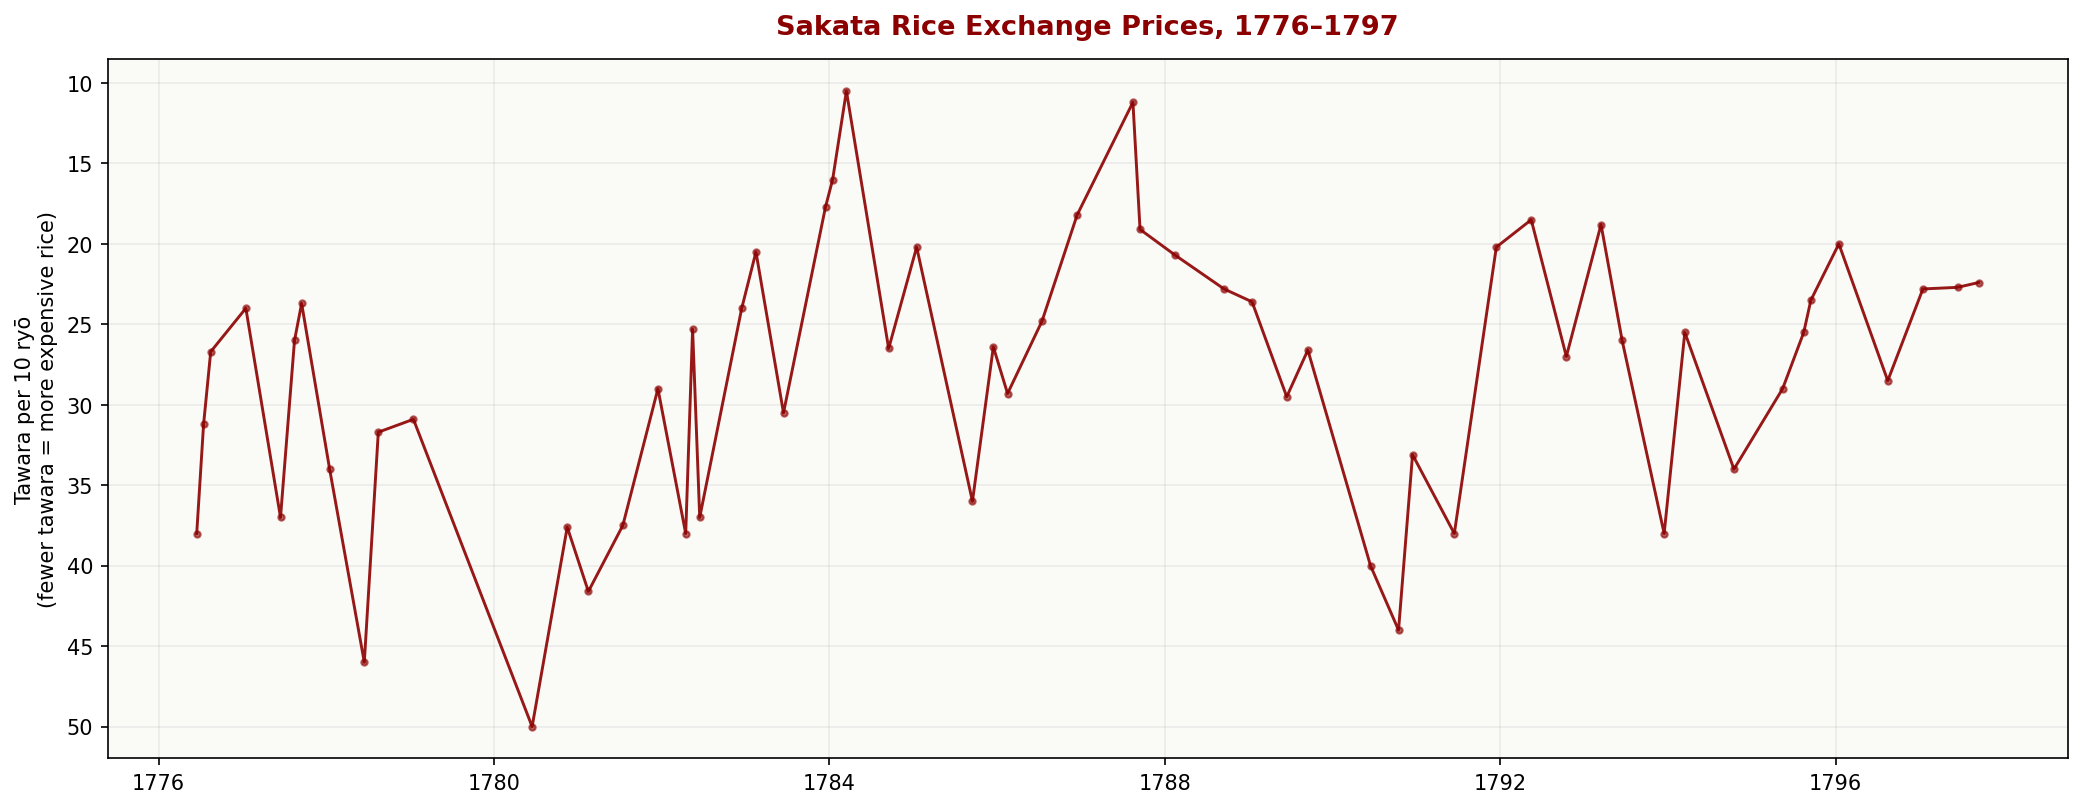
\includegraphics[width=\textwidth]{price_chart.png}
\caption{Sakata rice prices, An'ei 5 (1776) through Kansei 9 (1797),
reconstructed from the records in Article~85. The mean-reverting
character of the market is visible: prices oscillate within a bounded
range, with each spike followed by a return toward the center.}
\end{figure}

% --- An'ei 5 (1776) ---
\subsection*{An'ei 5, Year of the Monkey\hfill\normalfont\small\jp{安永五申年} (1776)}

Year-block direction: west (\jp{塞午}).
First-stem month: 5th month (\jp{五月甲}).
Autumn harvest: six-tenths crop (\jt{六分作}{rokubun-saku}).

\begin{description}[style=nextline, leftmargin=2em, font=\normalfont\bfseries]
\item[Opening] 38 tawara
\item[5th month (\textit{kinoe})] 31 tawara, 2 bu
\item[5th month] 26 tawara, 7 bu --- approximately 140-tawara rise
\item[6th month] 26 tawara, 7 bu --- 41-tawara decline
\item[12th month, 2nd day] 24 tawara --- \textit{kanoto} ceiling, 140-tawara rise
\end{description}

% --- An'ei 6 (1777) ---
\subsection*{An'ei 6, Year of the Rooster\hfill\normalfont\small\jp{安永六酉年} (1777)}

\begin{description}[style=nextline, leftmargin=2em, font=\normalfont\bfseries]
\item[Opening] 37 tawara
\item[6th month] 26 tawara
\item[7th month] 23 tawara, 7 bu
\item[Through 12th month] around 34 tawara
\end{description}

% --- An'ei 7 (1778) ---
\subsection*{An'ei 7, Year of the Dog\hfill\normalfont\small\jp{安永七戌年} (1778)}

Year-block direction: west (\jp{塞午}).
First-stem month: 11th month (\jp{十一月甲}).

\begin{description}[style=nextline, leftmargin=2em, font=\normalfont\bfseries]
\item[Opening] 46 tawara
\item[1st month] 31 tawara, 7 bu --- noted as ``sign of a \textit{kinoe} rise''
\item[1st month onward] A dispute arose at the certificate office (\jp{札方へ申分出}); 35 tawara, 5 bu. No settlement through the 10th month.
\item[11th month (\textit{kinoe})] 30 tawara, 9 bu --- ceiling on a \textit{fuj\=ojunichi}, 151-tawara rise
\end{description}

\textit{Following year, Year of the Boar:}
\begin{description}[style=nextline, leftmargin=2em, font=\normalfont\bfseries]
\item[6th month] 35 tawara, 5 bu --- 46-tawara decline
\end{description}

% --- An'ei 8 (1779) ---
\subsection*{An'ei 8, Year of the Boar\hfill\normalfont\small\jp{安永八亥年} (1779)}

Year-block direction: west (\jp{塞西}).

\begin{description}[style=nextline, leftmargin=2em, font=\normalfont\bfseries]
\item[Opening] 39 tawara to 44 tawara, 5 bu (range)
\item[Note] A dispute arose at the certificate office; no trading.
\end{description}

% --- An'ei 9 (1780) ---
\subsection*{An'ei 9, Year of the Rat\hfill\normalfont\small\jp{安永九子年} (1780)}

Year-block: west, rotating to Rooster (\jp{寒酉}).
First-stem month: 7th month (\jp{七月甲}).

This year's goods were plentiful; physical rice also at 50 tawara. New
certificates also opened at 50 tawara.

\begin{description}[style=nextline, leftmargin=2em, font=\normalfont\bfseries]
\item[9th month] 37 tawara, 6 bu
\end{description}

\textit{Following year, Year of the Ox:}
\begin{description}[style=nextline, leftmargin=2em, font=\normalfont\bfseries]
\item[1st month] 41 tawara, 6 bu
\item[5th month] 35 tawara, 9 bu --- ceiling on a \textit{hassen-k\=o}, 57-tawara rise
\end{description}

% --- Tenmei 1 (1781) ---
\subsection*{Tenmei 1, Year of the Ox\hfill\normalfont\small\jp{天明元丑年} (1781)}

Year-block: west (\jp{塞西}).
First-stem month: 5th month (\jp{五月甲}).

\begin{description}[style=nextline, leftmargin=2em, font=\normalfont\bfseries]
\item[5th month] 37 tawara, 5 bu
\item[10th month, 18th day] 29 tawara --- 188-tawara rise
\end{description}

\textit{Following year, Year of the Tiger:}
\begin{description}[style=nextline, leftmargin=2em, font=\normalfont\bfseries]
\item[3rd month] 38 tawara
\item[3rd month] 25 tawara, 3 bu --- \textit{kinoe} ceiling on an ordinary day, cumulative 127-tawara rise
\item[7th month] 25 tawara, 3 bu
\item[7th month] 27 tawara, 7 bu --- 24-tawara decline
\end{description}

% --- Tenmei 2 (1782) ---
\subsection*{Tenmei 2, Year of the Tiger\hfill\normalfont\small\jp{天明二寅年} (1782)}

Year-block: Rat direction (\jp{塞子}).
First-stem month: 3rd month (\jp{三月甲}).

\begin{description}[style=nextline, leftmargin=2em, font=\normalfont\bfseries]
\item[Opening] 37 tawara
\item[10th month] 24 tawara --- ceiling on a \textit{fuj\=ojunichi}, 130-tawara rise
\end{description}

\textit{Following year, Year of the Rabbit:}
\begin{description}[style=nextline, leftmargin=2em, font=\normalfont\bfseries]
\item[1st month] 20 tawara, 5 bu --- \textit{kinoe} ceiling, cumulative 33 tawara, 5 bu
\end{description}

% --- Tenmei 3 (1783) ---
\subsection*{Tenmei 3, Year of the Rabbit\hfill\normalfont\small\jp{天明三卯年} (1783)}

Year-block: Rat direction (\jp{塞子}).
First-stem month: 1st month (\jp{正月甲}).

\begin{description}[style=nextline, leftmargin=2em, font=\normalfont\bfseries]
\item[Opening] 30 tawara, 5 bu
\item[10th month] 17 tawara, 7 bu --- from 17.5 tawara
\item[12th month] 16 tawara
\end{description}

\textit{Following year, Year of the Dragon:}
\begin{description}[style=nextline, leftmargin=2em, font=\normalfont\bfseries]
\item[1st month, 2nd day] 12 tawara, 8 bu
\item[1st month, 26th day] 10 tawara, 5 bu --- \textit{hinoe} ceiling, 200-tawara rise
\item[7th month] 26 tawara, 5 bu --- 160-tawara decline
\end{description}

% --- Tenmei 4 (1784) ---
\subsection*{Tenmei 4, Year of the Dragon\hfill\normalfont\small\jp{天明四辰年} (1784)}

Year-block: blocked-Ox (\jp{塞子}).
First-stem month: 9th month (\jp{九月甲}).

\begin{description}[style=nextline, leftmargin=2em, font=\normalfont\bfseries]
\item[Opening] 32 tawara, 5 bu
\item[7th month (\textit{kinoe})] 20 tawara, 2 bu
\item[12th month] 20 tawara, 2 bu --- \textit{hinoto} ceiling, 123-tawara rise
\end{description}

% --- Tenmei 5 (1785) ---
\subsection*{Tenmei 5, Year of the Snake\hfill\normalfont\small\jp{天明五巳年} (1785)}

Year-block: blocked-Rabbit (\jp{塞卯}).
First-stem month: 7th month (\jp{七月甲}).

\begin{description}[style=nextline, leftmargin=2em, font=\normalfont\bfseries]
\item[7th month] 36 tawara
\item[10th month] 26 tawara, 4 bu --- \textit{ushi}-day \textit{hinoto} rise, 96-tawara rise
\item[12th month] 28 tawara, 8 bu
\end{description}

\textit{Following year, Year of the Horse:}
\begin{description}[style=nextline, leftmargin=2em, font=\normalfont\bfseries]
\item[1st month] 29 tawara, 3 bu
\item[5th month] 24 tawara, 8 bu --- \textit{ushi}-day \textit{kinoto} ceiling, total 116-tawara rise
\item[6th month] 24 tawara, 8 bu
\end{description}

% --- Tenmei 6 (1786) ---
\subsection*{Tenmei 6, Year of the Horse\hfill\normalfont\small\jp{天明六午年} (1786)}

Year-block: blocked-Rabbit (\jp{塞卯}).
First-stem month: 5th month (\jp{五月甲}).

\begin{description}[style=nextline, leftmargin=2em, font=\normalfont\bfseries]
\item[Opening] 30 tawara, 5 bu
\item[Same month] 18 tawara, 2 bu --- 5-tawara rise
\item[10th month] 18 tawara, 2 bu
\end{description}

\textit{Following year, Year of the Sheep:}
\begin{description}[style=nextline, leftmargin=2em, font=\normalfont\bfseries]
\item[6th month] 11 tawara, 2 bu --- \textit{fuj\=ojitsu}-day \textit{hinoto} ceiling, total 193-tawara rise
\item[Same month] 19 tawara, 1 bu --- 79-tawara decline
\end{description}

% --- Tenmei 7 (1787) ---
\subsection*{Tenmei 7, Year of the Sheep\hfill\normalfont\small\jp{天明七未年} (1787)}

Year-block: blocked-Rabbit (\jp{塞卯}).
First-stem month: 3rd month (\jp{三月甲}).

\begin{description}[style=nextline, leftmargin=2em, font=\normalfont\bfseries]
\item[Opening] 27 tawara
\end{description}

\textit{Following year, Year of the Monkey:}
\begin{description}[style=nextline, leftmargin=2em, font=\normalfont\bfseries]
\item[1st month] 20 tawara, 7 bu --- \textit{kinoe} ceiling, 63-tawara rise
\item[7th/8th month] 22 tawara, 8 bu
\item[9th month] 26 tawara
\end{description}

% --- Tenmei 8 (1788) ---
\subsection*{Tenmei 8, Year of the Monkey\hfill\normalfont\small\jp{天明八申年} (1788)}

Year-block: blocked-Horse (\jp{塞午}).
First-stem month: 1st month (\jp{正月甲}).

\begin{description}[style=nextline, leftmargin=2em, font=\normalfont\bfseries]
\item[Opening] 26 tawara
\item[11th month] 23 tawara, 6 bu --- \textit{ushi}-day \textit{kinoe} ceiling, 24-tawara rise
\end{description}

\textit{Following year, Year of the Rooster:}
\begin{description}[style=nextline, leftmargin=2em, font=\normalfont\bfseries]
\item[6th month] 40 tawara, 5 bu
\end{description}

% --- Tenmei 9 / Kansei 1 (1789) ---
\subsection*{Tenmei 9 / Kansei 1, Year of the Rooster\hfill\normalfont\small\jp{天明九酉年} (1789)}

Era changed to Kansei (\jp{寛政と改元}).
Year-block: blocked-Horse (\jp{塞午}).
First-stem month: 11th month (\jp{十一月甲}).

\begin{description}[style=nextline, leftmargin=2em, font=\normalfont\bfseries]
\item[Opening] 29 tawara, 5 bu
\item[7th month] 26 tawara, 6 bu
\item[Note] The record breaks off here.
\end{description}

% --- Kansei 2 (1790) ---
\subsection*{Kansei 2, Year of the Dog\hfill\normalfont\small\jp{寛政二戌年} (1790)}

Year-block: blocked-Horse (\jp{塞午}).
First-stem month: 7th month (\jp{七月甲}).

\begin{description}[style=nextline, leftmargin=2em, font=\normalfont\bfseries]
\item[New opening] 40 tawara
\item[8th month] 44 tawara
\item[10th month] 33 tawara, 1 bu --- \textit{kinoto} ceiling
\end{description}

% --- Kansei 3 (1791) ---
\subsection*{Kansei 3, Year of the Boar\hfill\normalfont\small\jp{寛政三亥年} (1791)}

Year-block: blocked-Rooster (\jp{塞酉}).
First-stem month: 5th month (\jp{五月甲}).

\begin{description}[style=nextline, leftmargin=2em, font=\normalfont\bfseries]
\item[Opening] 38 tawara --- from 27 tawara, 2 bu
\item[10th month] 20 tawara, 2 bu --- \textit{ten'ichi ten'j\=o}-day, 178-tawara rise
\item[12th month] 24 tawara
\end{description}

\textit{Following year, Year of the Rat:}
\begin{description}[style=nextline, leftmargin=2em, font=\normalfont\bfseries]
\item[3rd month, 16th day] 18 tawara, 5 bu --- 87-tawara decline
\item[6th month] 18 tawara, 9 bu --- 81-tawara decline
\item[8th month] 27 tawara --- rises again; 22 tawara
\end{description}

% --- Kansei 4 (1792) ---
\subsection*{Kansei 4, Year of the Rat\hfill\normalfont\small\jp{寛政四子年} (1792)}

Year-block: blocked-Rooster (\jp{塞酉}).
First-stem month: 3rd month (\jp{三月甲}).

\begin{description}[style=nextline, leftmargin=2em, font=\normalfont\bfseries]
\item[New opening] 32 tawara, 9 bu
\item[9th month] 22 tawara, 4 bu --- \textit{ten'ichi ten'j\=o} rise
\item[12th month] 23 tawara, 3 bu
\end{description}

\textit{Following year, Year of the Ox:}
\begin{description}[style=nextline, leftmargin=2em, font=\normalfont\bfseries]
\item[1st month, 17th day] 18 tawara, 8 bu --- \textit{kinoe} ceiling, total 148-tawara rise
\end{description}

% --- Kansei 5 (1793) ---
\subsection*{Kansei 5, Year of the Ox\hfill\normalfont\small\jp{寛政五丑年} (1793)}

Year-block: blocked-Rooster (\jp{塞酉}).
First-stem month: 1st month (\jp{正月甲}).

\begin{description}[style=nextline, leftmargin=2em, font=\normalfont\bfseries]
\item[New opening] 26 tawara
\item[Up to 10th month, 8th day] 38 tawara
\item[11th month] 31 tawara
\item[12th month] 30 tawara, 2 bu
\end{description}

\textit{Following year, Year of the Tiger:}
\begin{description}[style=nextline, leftmargin=2em, font=\normalfont\bfseries]
\item[1st month] 25 tawara, 5 bu --- \textit{ten'ichi ten'j\=o}-day \textit{hinoe} ceiling, 125-tawara rise
\item[6th month] 29 tawara
\item[8th month] 34 tawara --- 85-tawara decline
\end{description}

% --- Kansei 6 (1794) ---
\subsection*{Kansei 6, Year of the Tiger\hfill\normalfont\small\jp{寛政六寅年} (1794)}

Year-block: blocked-Rat (\jp{塞子}).
First-stem month: 9th month (\jp{九月甲}).

\begin{description}[style=nextline, leftmargin=2em, font=\normalfont\bfseries]
\item[New opening] 32 tawara
\item[8th month] 28 tawara, 3 bu
\end{description}

\textit{Following year, Year of the Rabbit:}
\begin{description}[style=nextline, leftmargin=2em, font=\normalfont\bfseries]
\item[Through 3rd month] Consolidation (\jp{持合})
\item[4th month onward] Around 29 tawara
\item[6th/7th month] Around 25 tawara, 5 bu --- \textit{kinoe} ceiling, approximately 65-tawara rise
\end{description}

% --- Kansei 7 (1795) ---
\subsection*{Kansei 7, Year of the Rabbit\hfill\normalfont\small\jp{寛政七卯年} (1795)}

Year-block: blocked-Rat (\jp{塞子}).
First-stem month: 7th month (\jp{七月甲}).

\begin{description}[style=nextline, leftmargin=2em, font=\normalfont\bfseries]
\item[New opening] 31 tawara
\item[7th month, 23rd day] 23 tawara, 5 bu --- \textit{ushi}-day \textit{tsuchinoe} ceiling, 128-tawara rise
\item[12th month] 20 tawara
\end{description}

\textit{Following year, Year of the Dragon:}
\begin{description}[style=nextline, leftmargin=2em, font=\normalfont\bfseries]
\item[1st--3rd month] From 19 tawara, around 20 tawara
\item[6th month, 22nd--23rd day] 28 tawara, 5 bu --- floor, 102-tawara decline
\item[Thereafter] Rises again to around 23.5 tawara
\end{description}

% --- Kansei 8 (1796) ---
\subsection*{Kansei 8, Year of the Dragon\hfill\normalfont\small\jp{寛政八辰年} (1796)}

Year-block: blocked-Rat (\jp{塞子}).
First-stem month: 5th month (\jp{五月甲}).

\begin{description}[style=nextline, leftmargin=2em, font=\normalfont\bfseries]
\item[Opening] 31 tawara, 4 bu
\item[11th month, 16th day] 22 tawara, 8 bu --- \textit{ushi}-day \textit{kanoe}, 87-tawara rise
\end{description}

\textit{Following year, Year of the Snake:}
\begin{description}[style=nextline, leftmargin=2em, font=\normalfont\bfseries]
\item[4th month, 29th day] 22 tawara, 7 bu --- 36-tawara decline
\item[7th month, 19th day] 22 tawara, 4 bu --- \textit{ushi}-day \textit{tsuchinoto} rise
\item[Intercalary 7th month] Record ends.
\end{description}

\bigskip

\begin{editorialnote}
The foregoing records the price movements of the Sakata rice exchange. In
the lower line, annotations such as ``\textit{kinoe} ceiling'' (\jp{甲天井})
or ``\textit{hinoe} ceiling'' (\jp{丙天井}) mean that the market reached its
ceiling in a \textit{kinoe}-month or a \textit{hinoe}-month, respectively.
The figures ``rise of one hundred and some-odd tawara'' (\jp{百何十俵上})
that follow are stated per 100 ry\=o of capital.
\end{editorialnote}

% =============================================================================
%  END OF LOWER VOLUME
% =============================================================================

\begin{center}
\rule{2in}{0.4pt}\\[1em]
{\small\itshape End of the Lower Volume}\\[0.3em]
{\small \jp{宗久翁相塲全集終}}
\end{center}
